\documentclass[11pt]{article}
\usepackage{matt}
\begin{document}

\section*{Update for the Week of \today}

\begin{figure}[h]
  \centering
  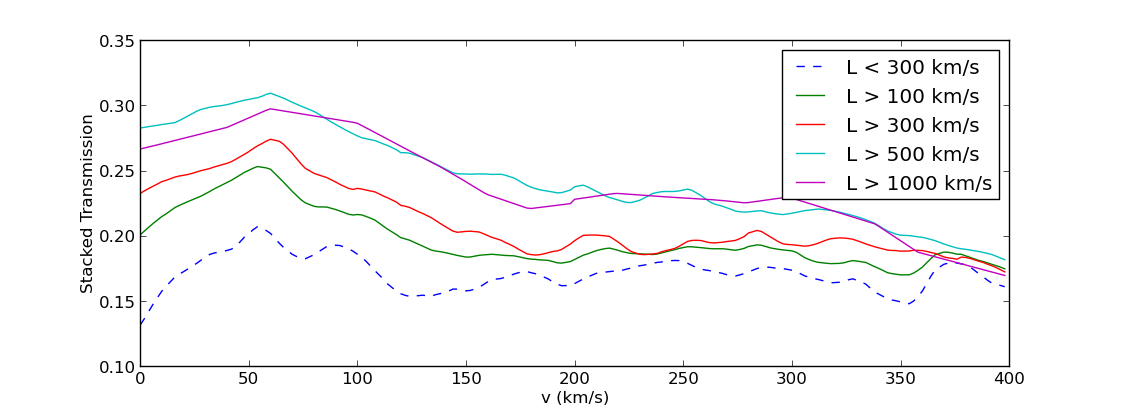
\includegraphics[width=18cm]{Stacks_Skip2ndSpectrum_NoWeighting.png}
  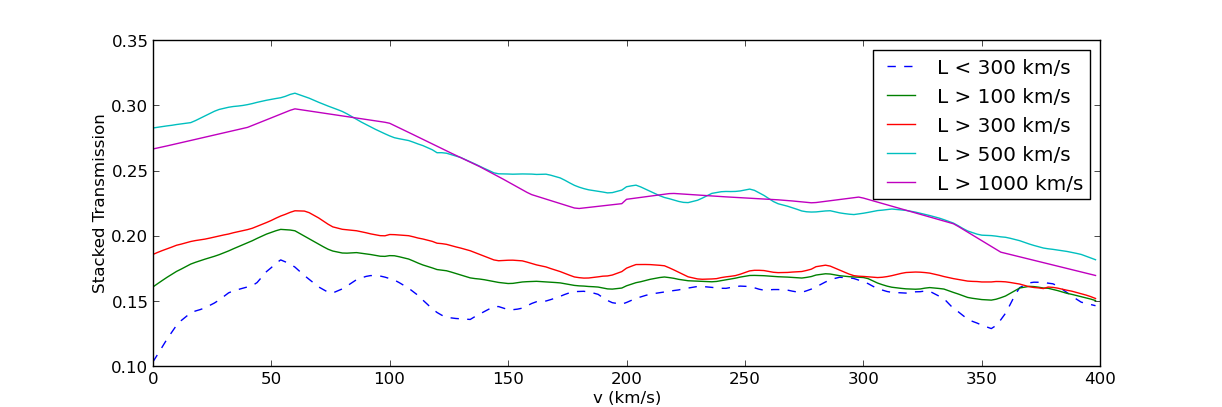
\includegraphics[width=18cm]{Stacks_Skip2ndSpectrum.png}
  \caption{The above figures are the same as Fig. \ref{fig:Stacks} except that we have excluded one of the spectrum from the stack. This spectrum, for whatever reason, had many more dark gaps than the others and had a large impact on the average. The left figure weights each spectrum the same while the right-hand figure weights spectra according to their signal-to-noise values. }
  \label{fig:SkipSome}
\end{figure}


\begin{figure}[h]
  \centering
  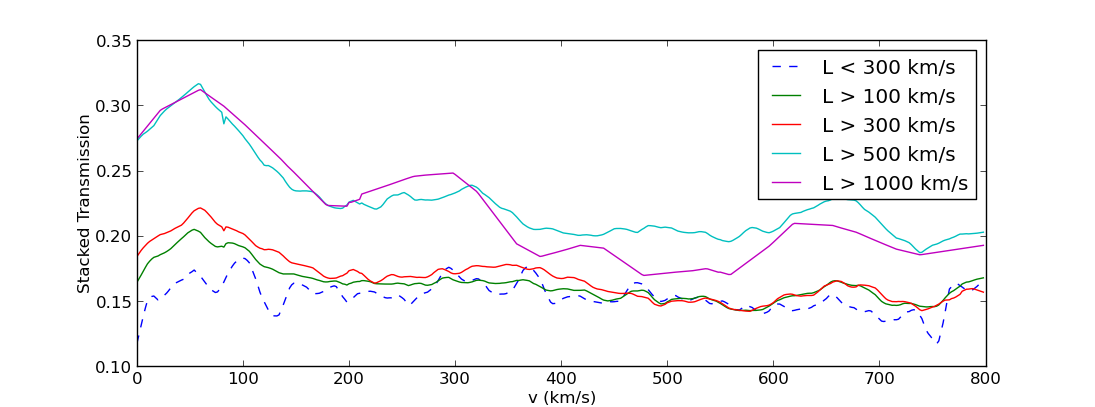
\includegraphics[width=18cm]{Stacks_Extended_NoWeighting.png}
  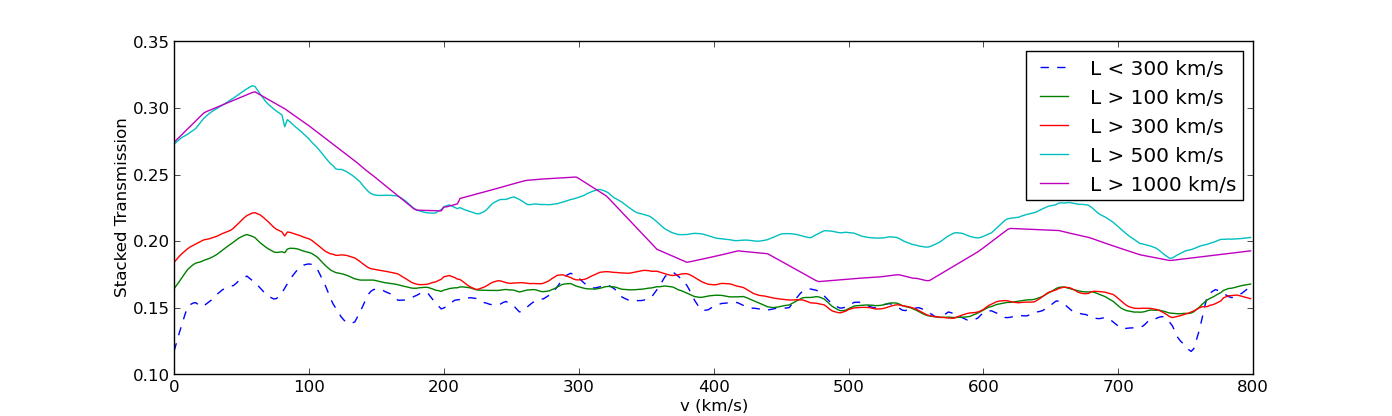
\includegraphics[width=18cm]{Stacks_Extended.png}
  \caption{The above figures are the same as in Fig. \ref{fig:SkipSome} except that we have extended the velocity range for the stack.}
  \label{fig:todo}
\end{figure}


\begin{figure}[h]
  \centering
  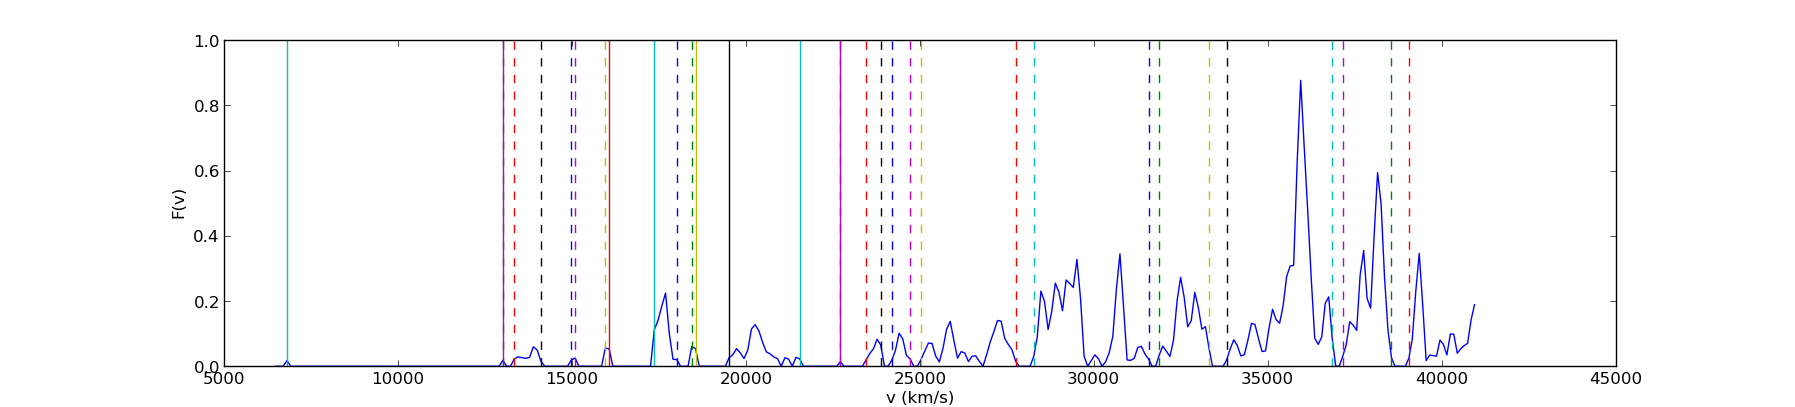
\includegraphics[width=18cm]{figure_1.png}
  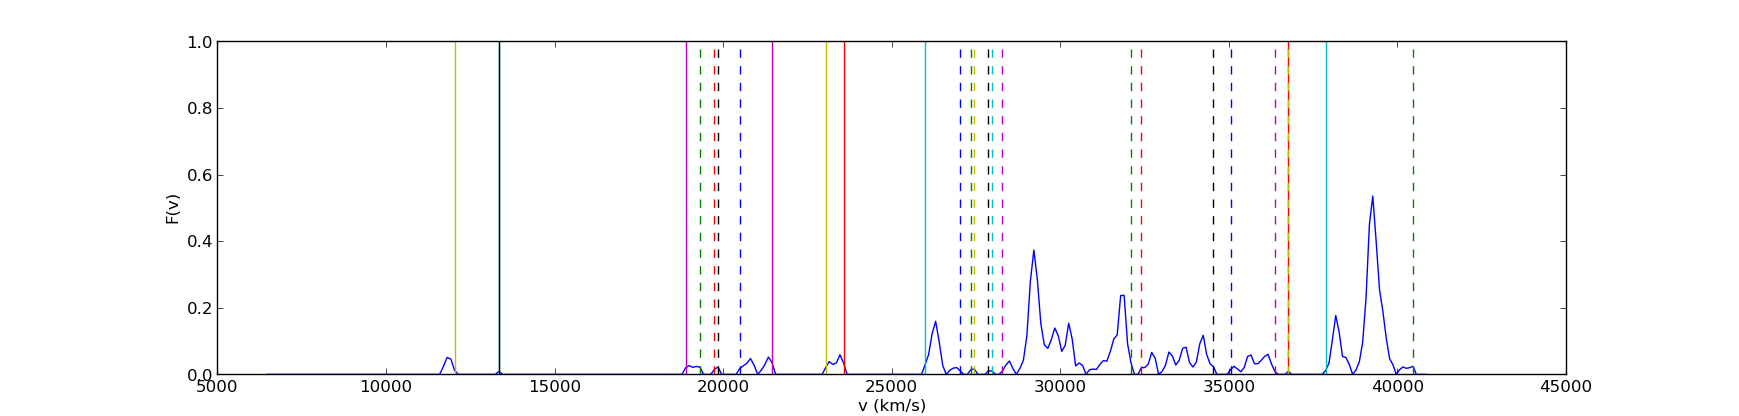
\includegraphics[width=18cm]{figure_2.png}
  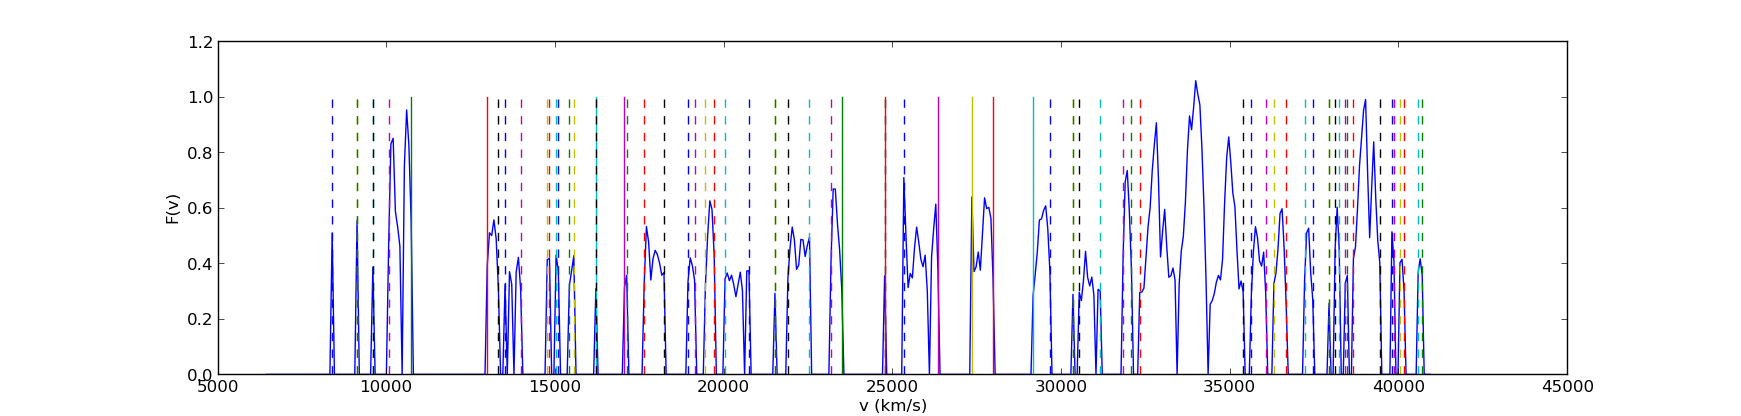
\includegraphics[width=18cm]{figure_3.png}
  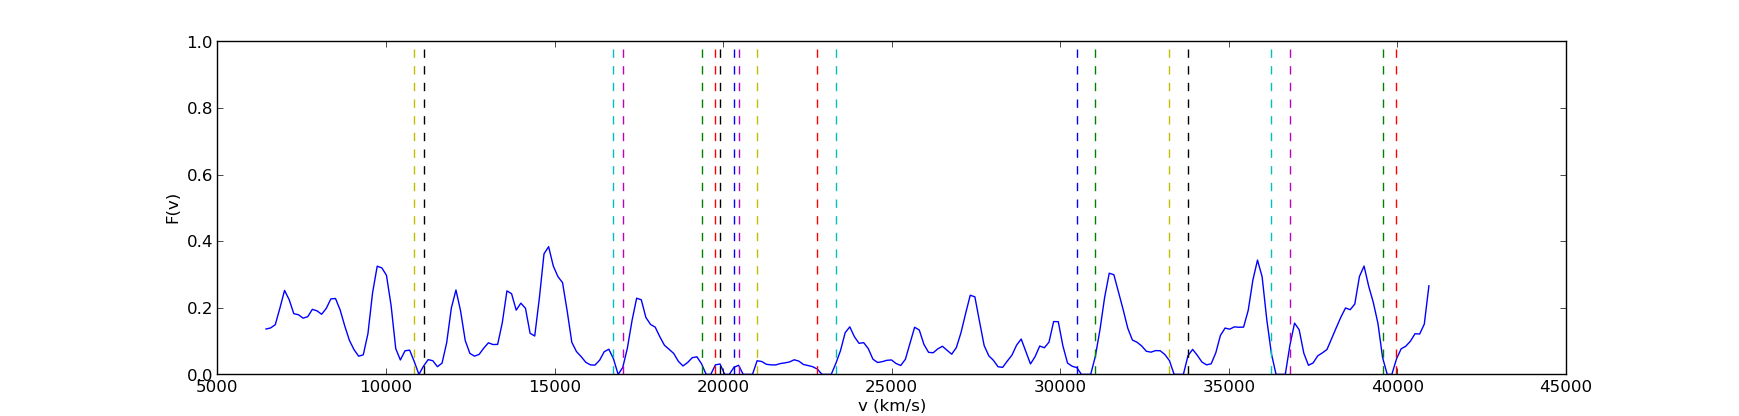
\includegraphics[width=18cm]{figure_4.png}
  \caption{The above figure shows 4 example spectra along with the detected stacking locations. Solid (dashed) lines indicate the boundaries of large (small) dark gaps where stacking occurs. The spectra have been smoothed over $\sim 100$km/s and regions with $F < 3\tilde{\sigma}_{\text{N}}$ have been set to zero. This is mainly to show stacking locations; the stacked transmission is taken from unsmoothed spectra.}
  \label{fig:todo}
\end{figure}

\begin{figure}[h]
  \centering
  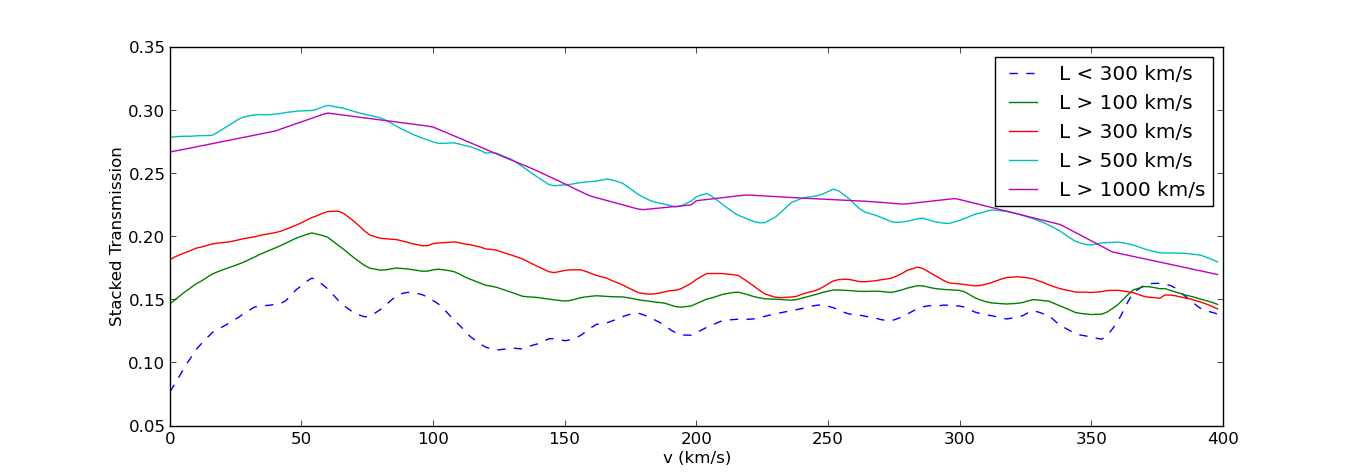
\includegraphics[width=18cm]{figure_5.png}
  \caption{The above figure shows the results of stacking spectra outside of large (solid) and small (dashed) dark gaps in our actual spectra. We show the stacking results for several values of minimum dark gap size. Contributions to the stacked transmission for each spectrum have been weighted by that spectra's signal-to-noise value as estimated by the signal standard deviation divided by the mean value in the region of the spectra that we use for the continuum fit.}
  \label{fig:Stacks}
\end{figure}



%\begin{figure}[h]
%  \centering
%  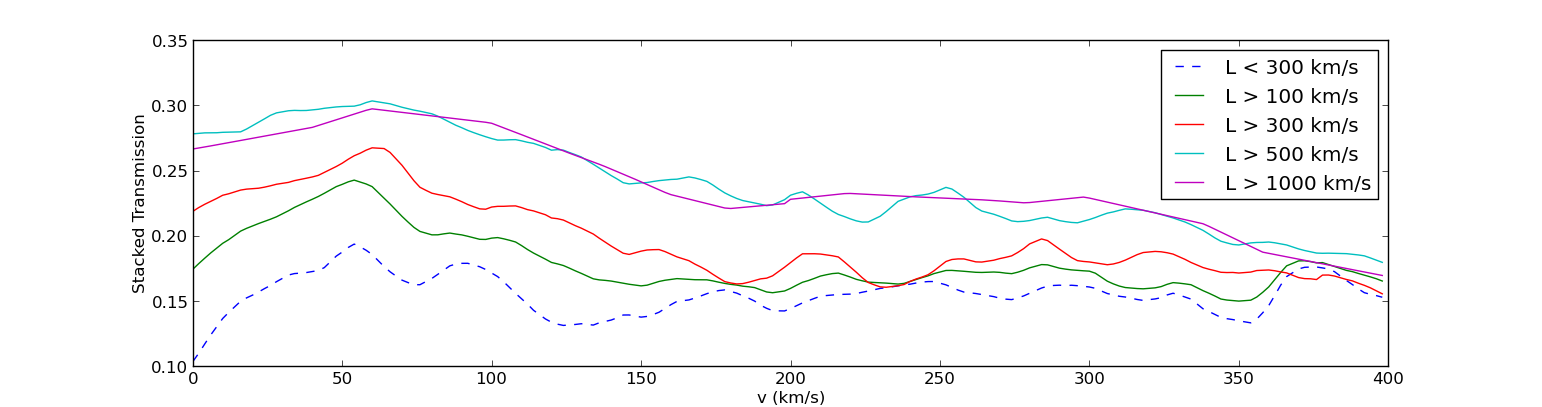
\includegraphics[width=18cm]{figure_6.png}
%  \caption{The above figure shows the results of stacking spectra outside of large (solid) and small (dashed) dark gaps in our actual spectra. We show the stacking results for several values of minimum dark gap size. In this figure, we weight contributions from each spectrum equally, regardless of the spectrum's signal to noise.}
%  \label{fig:todo}
%\end{figure}


\begin{figure}[h]
  \centering
  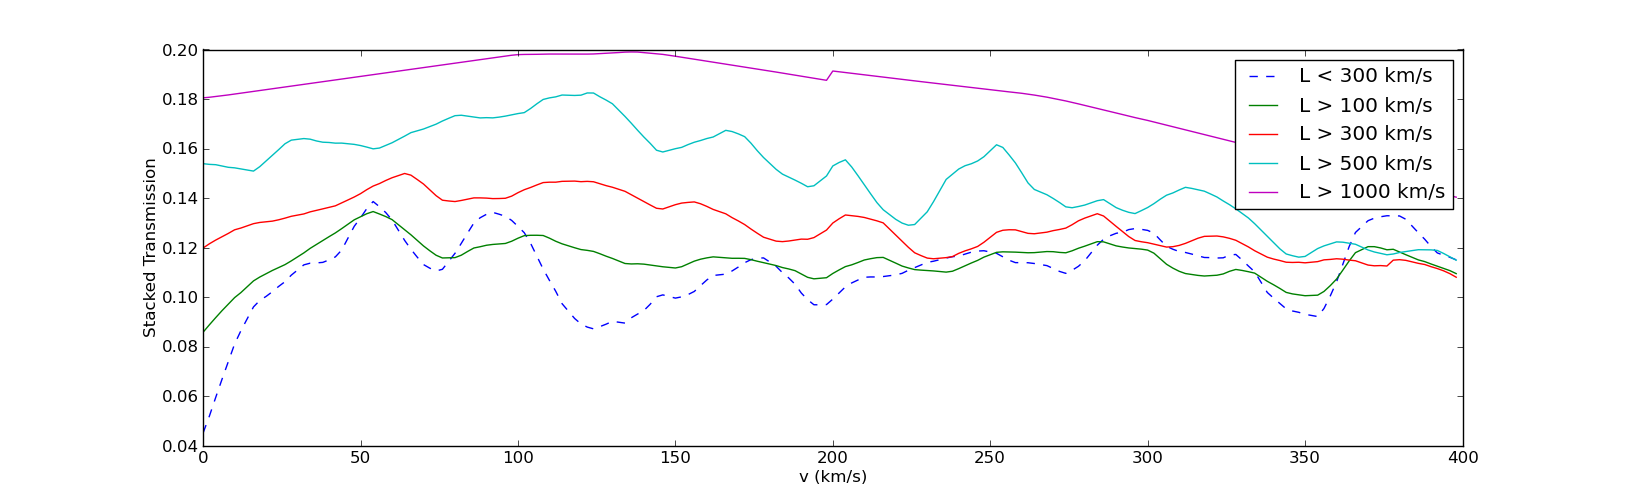
\includegraphics[width=8cm]{Stacks_ZGreaterThan5p5.png}
  \caption{The above figure is the same as Fig. \ref{fig:Stacks} except we only use quasars with $z _{\text{em}} \geq 5.5$.}
  \label{fig:todo}
\end{figure}


\end{document}